\hypertarget{dbprim__int_8h}{
\section{dbprim\_\-int.h File Reference}
\label{dbprim__int_8h}\index{dbprim_int.h@{dbprim\_\-int.h}}
}


\subsection{Detailed Description}
\begin{Desc}
\item[For internal use only.]
This file contains the \#define's and function declarations used internally by the Database Primitives Library.\end{Desc}


Definition in file \hyperlink{dbprim__int_8h-source}{dbprim\_\-int.h}.

{\tt \#include \char`\"{}dbprim\_\-err.h\char`\"{}}\par
{\tt \#include \char`\"{}dbprim\_\-version.h\char`\"{}}\par


Include dependency graph for dbprim\_\-int.h:\begin{figure}[H]
\begin{center}
\leavevmode
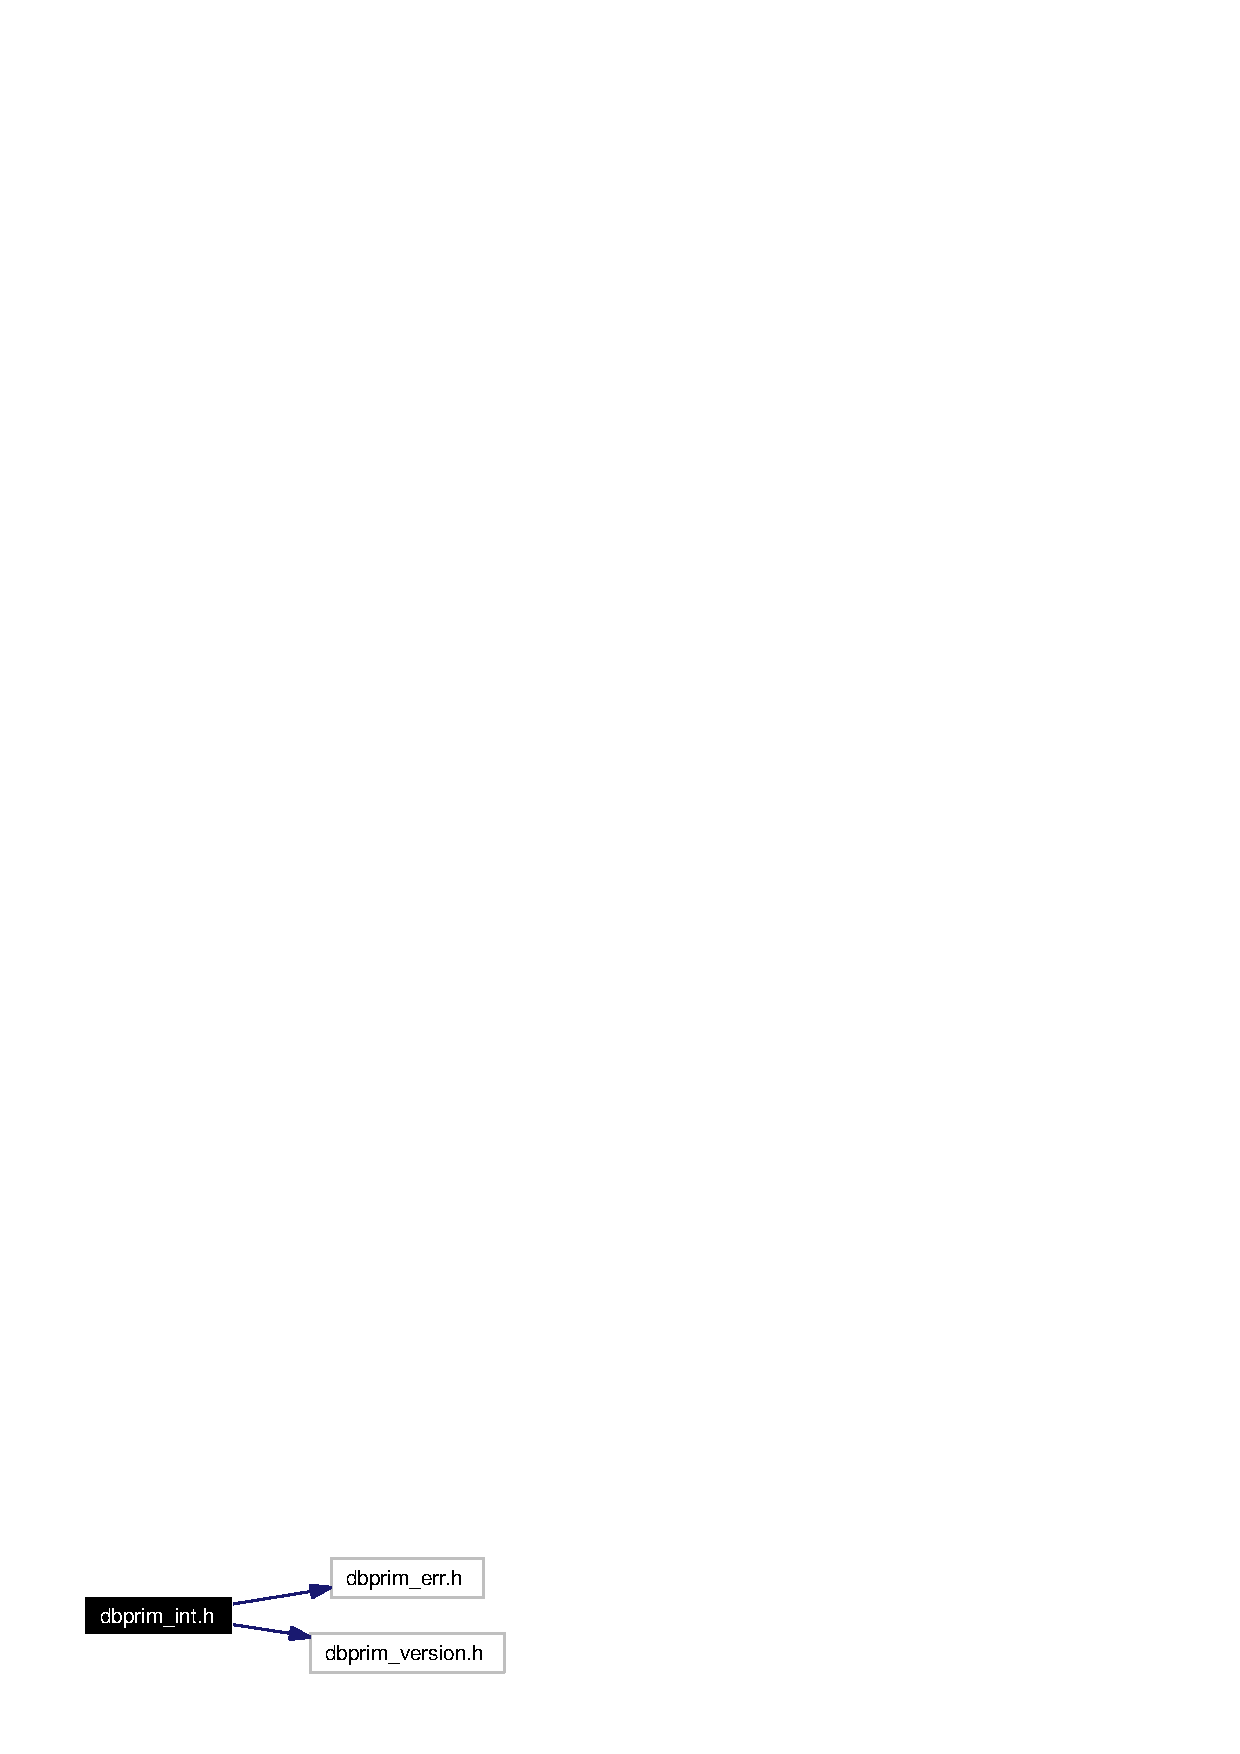
\includegraphics[width=123pt]{dbprim__int_8h__incl}
\end{center}
\end{figure}


This graph shows which files directly or indirectly include this file:\begin{figure}[H]
\begin{center}
\leavevmode
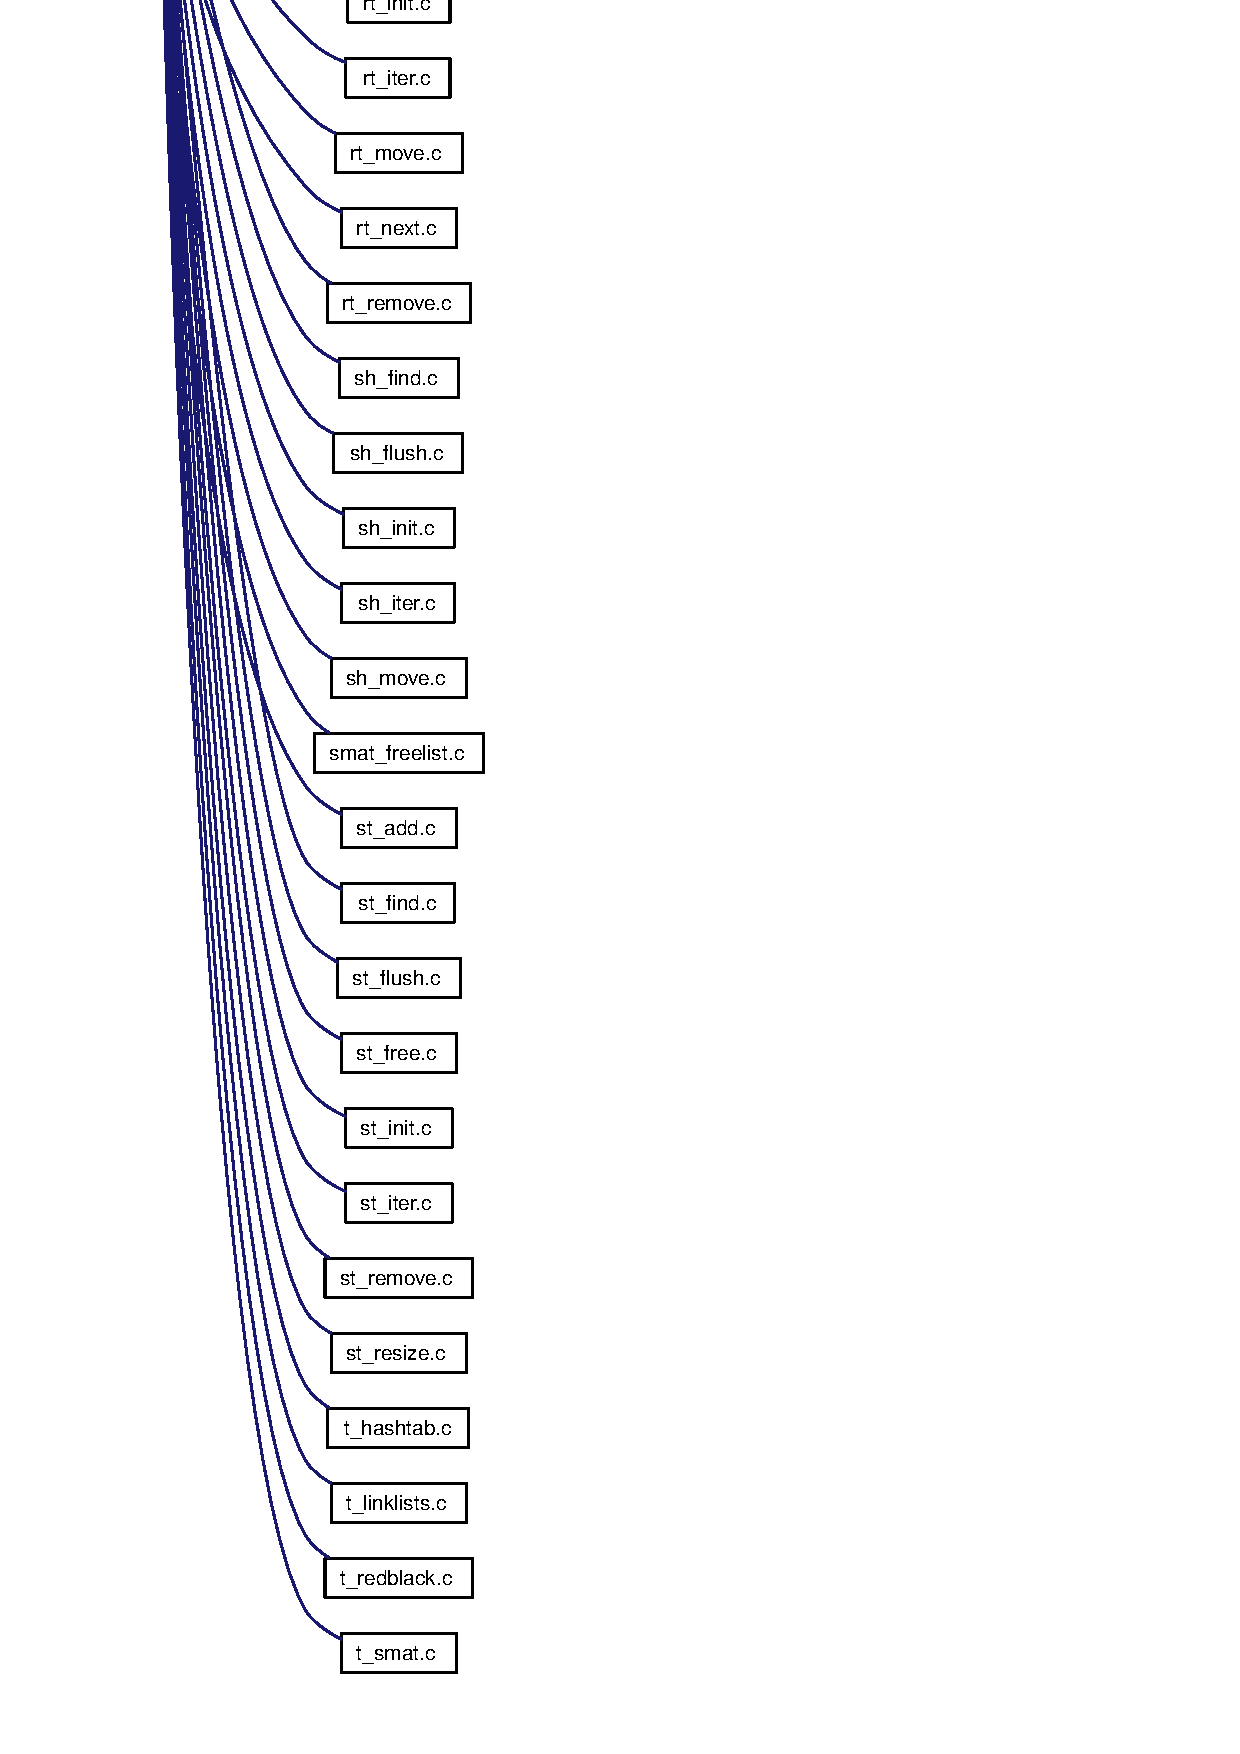
\includegraphics[width=119pt]{dbprim__int_8h__dep__incl}
\end{center}
\end{figure}
\subsection*{Defines}
\begin{CompactItemize}
\item 
\#define \hyperlink{dbprim__int_8h_a0}{RCSTAG}(tag)
\begin{CompactList}\small\item\em Embed RCS revision information. \item\end{CompactList}\item 
\#define \hyperlink{group__dbprim__hash_ga46}{\_\-hash\_\-rollover}(mod)
\begin{CompactList}\small\item\em Select hash table roll over size. \item\end{CompactList}\item 
\#define \hyperlink{group__dbprim__hash_ga47}{\_\-hash\_\-rollunder}(mod)
\begin{CompactList}\small\item\em Select hash table roll under size. \item\end{CompactList}\item 
\#define \hyperlink{group__dbprim__hash_ga48}{\_\-hash\_\-fuzz}(mod)
\begin{CompactList}\small\item\em Fuzz the initial hash table size. \item\end{CompactList}\item 
\#define \hyperlink{group__dbprim__hash_ga49}{HASH\_\-FNV\_\-OFFSET}
\begin{CompactList}\small\item\em FNV offset basis parameter. \item\end{CompactList}\item 
\#define \hyperlink{group__dbprim__hash_ga50}{HASH\_\-FNV\_\-PRIME}
\begin{CompactList}\small\item\em FNV prime parameter. \item\end{CompactList}\item 
\#define \hyperlink{group__dbprim__smat_ga66}{ST\_\-REM\_\-FIRST}
\begin{CompactList}\small\item\em Flag requesting removal from first list. \item\end{CompactList}\item 
\#define \hyperlink{group__dbprim__smat_ga67}{ST\_\-REM\_\-SECOND}
\begin{CompactList}\small\item\em Flag requesting removal from second list. \item\end{CompactList}\item 
\#define \hyperlink{group__dbprim__smat_ga68}{ST\_\-REM\_\-HASH}
\begin{CompactList}\small\item\em Flag requesting removal from hash table. \item\end{CompactList}\item 
\#define \hyperlink{group__dbprim__smat_ga69}{ST\_\-REM\_\-FREE}
\begin{CompactList}\small\item\em Flag requesting memory release. \item\end{CompactList}\end{CompactItemize}
\subsection*{Functions}
\begin{CompactItemize}
\item 
unsigned long \hyperlink{group__dbprim__hash_ga19}{\_\-hash\_\-prime} (unsigned long start)
\begin{CompactList}\small\item\em Select a prime number. \item\end{CompactList}\item 
unsigned long \hyperlink{group__dbprim__smat_ga24}{\_\-st\_\-remove} (\hyperlink{struct__smat__table__s}{smat\_\-table\_\-t} $\ast$table, \hyperlink{struct__smat__entry__s}{smat\_\-entry\_\-t} $\ast$entry, unsigned int remflag)
\begin{CompactList}\small\item\em Remove an entry from a sparse matrix (internal). \item\end{CompactList}\item 
\hyperlink{struct__smat__entry__s}{smat\_\-entry\_\-t} $\ast$ \hyperlink{group__dbprim__smat_ga25}{\_\-smat\_\-alloc} (void)
\begin{CompactList}\small\item\em Allocate a sparse matrix entry. \item\end{CompactList}\item 
void \hyperlink{group__dbprim__smat_ga26}{\_\-smat\_\-free} (\hyperlink{struct__smat__entry__s}{smat\_\-entry\_\-t} $\ast$entry)
\begin{CompactList}\small\item\em Release a sparse matrix entry. \item\end{CompactList}\item 
\hyperlink{struct__rb__node__s}{rb\_\-node\_\-t} $\ast$ \hyperlink{group__dbprim__rbtree_ga14}{\_\-rb\_\-locate} (\hyperlink{struct__rb__tree__s}{rb\_\-tree\_\-t} $\ast$tree, \hyperlink{struct__rb__node__s}{rb\_\-node\_\-t} $\ast$node, \hyperlink{struct__db__key__s}{db\_\-key\_\-t} $\ast$key)
\begin{CompactList}\small\item\em Locate or insert a red-black tree node. \item\end{CompactList}\item 
void \hyperlink{group__dbprim__rbtree_ga15}{\_\-rb\_\-rotate} (\hyperlink{struct__rb__tree__s}{rb\_\-tree\_\-t} $\ast$tree, \hyperlink{struct__rb__node__s}{rb\_\-node\_\-t} $\ast$child)
\begin{CompactList}\small\item\em Rotate tree nodes. \item\end{CompactList}\end{CompactItemize}


\subsection{Define Documentation}
\hypertarget{dbprim__int_8h_a0}{
\index{dbprim_int.h@{dbprim\_\-int.h}!RCSTAG@{RCSTAG}}
\index{RCSTAG@{RCSTAG}!dbprim_int.h@{dbprim\_\-int.h}}
\subsubsection[RCSTAG]{\setlength{\rightskip}{0pt plus 5cm}\#define RCSTAG(tag)}}
\label{dbprim__int_8h_a0}


\begin{Desc}
\item[For internal use only.]
Embeds the {\tt tag} (a string including the RCS Id tag) into the binary. This can be useful when tracking down version skew issues.\end{Desc}


Definition at line 50 of file dbprim\_\-int.h.